%!TEX root = ../../dissertation.tex
\begin{savequote}[75mm]
I think it would be a good idea!
\qauthor{Mahatma Gandhi}
\end{savequote}
\chapter{Baseline Absolute Binding Free Energy Calculations: Sampling Methods and System Setup}
\label{ch:benchmarking-and-system-preparation}
\section{Introduction}


\subsection{Choosing Protocol:}



Out of the studies mentioned, we see that the different FEP studies have employed different sampling protocols. Lenselink et al. and Cappel et al. applied REST-enhanced RBFEs to GPCRs, and Guo et al. used REST2 for [RBFE/ABFE]. Vögele et al. went further for GPCR ABFEs by combining REST2 with GCMC water sampling (PMC). Baumann et al. introduced ε-HREX within their separated-topologies RBFE approach, softening ligand Lennard-Jones interactions to lower conformational barriers and improve sampling of slow ligand rotamers (PMC). Cook et al. instead initialised weakly coupled ABFE windows from apo conformations to address slow receptor relaxation after ligand decoupling (ChemRxiv). 
As these strategies target distinct sampling limitations, their relative merits for GPCR ABFE calculations remain unclear. We therefore do an initial benchmark and compare four protocol variants: HREX, ε-HREX, apo-initialised windows, and independent windows without HREX. The A2A receptor dataset of Lenselink et al. was selected as the test system, as it achieved the the highest R² among the GPCR RBFE benchmarks reported in Guo et al.

\subsection{System setup practices: Sodium}
In addition to sampling protocols, we examined how system preparation affects the calculations. Because we used input structures from the Guo et al. dataset, which were already optimised for RBFE performance, binding pocket issues were largely avoided. However, we noticed other issues, such as the treatment of ions.

The dataset contains six class A receptors (OX2R, TAAR1, A2A, D3, DOR and β1AR) and one class C receptor (mGlu5). Class A receptors are known to have a buried allosteric Na⁺ pocket centred on Asp²·⁵⁰, formed with other polar residues and coordinating waters. Class C receptors such as mGlu5 have a different transmembrane architecture and a large extracellular Venus-flytrap domain, with no known sodium-binding site.

Evidence for ion binding is strongest for A2A, DOR and β1AR, where high-resolution X-ray structures directly resolve Na⁺ in the conserved transmembrane pocket, supported by biochemical or biophysical experiments. For D3, evidence for sodium modulation of ligand affinity comes only from functional and ligand-binding experiments, in which mutations in the proposed sodium-binding network alter receptor responses or abolish sodium sensitivity. For OX2R, binding assays showed no significant sodium effect on EMPA binding, consistent with the absence of a resolved sodium ion in its structure. In mGlu5, the extracellular-domain structure (PDB 3LMK, 2.44 Å) contains a site modelled as Mg²⁺, but its identity and physiological significance require further validation.

Molecular dynamics simulations have probed sodium coordination and its coupling to receptor conformation and ligand recognition in A2A, D3 and DOR, providing mechanistic support, especially for D3, where sodium binding has not been structurally resolved. For TAAR1, receptor-specific evidence for ion binding remains insufficient in the literature we examined.

As a consequence of this uneven experimental characterisation, the treatment of ions during system preparation for free-energy perturbation (FEP) calculations varies across studies. Some computational protocols explicitly include ions in the binding pocket (2, 13), whereas others omit them (21), particularly when reasonable agreement with experiment is obtained without them. This variability is evident in the calculations of Guo et al. The A2A receptor systems with ligands from Minetti, Piersanti and Deflorian explicitly included the Na⁺ ion, whereas those from Lenselink et al. did not. Notably, despite the absence of sodium, the Lenselink data set showed the highest correlation with experimental binding affinities (R² = 0.84) of all the data sets analysed by Guo et al. Motivated by this apparent inconsistency, we systematically evaluated the impact of the allosteric sodium ion by performing absolute binding free energy calculations with and without Na⁺. Given the varying levels of evidence for Na⁺ binding across these receptors and our limited computational capacity, we restricted our analysis to systems where the treatment of sodium was ambiguous or inconsistent.

Three systems were selected to span the range of evidential support for sodium binding. A2A was chosen because Guo et al. treated sodium inconsistently across its ligand sets, including Na⁺ for some and omitting it for the Lenselink set, despite crystallographic evidence for its binding. D3 was included because the evidence for sodium modulation is exclusively functional, with no structural confirmation, leaving the role of the ion ambiguous. Finally, OX2R was selected because no evidence of sodium binding has been reported, yet it was simulated with Na⁺ present in the Guo et al. dataset.


\begin{table}[htbp]
    \centering
    \caption{Evidence supporting allosteric Na$^{+}$ binding in the
    investigated GPCRs. Functional evidence denotes sodium-dependent
    changes in ligand binding or signalling; structural evidence denotes
    Na$^{+}$ assigned in an experimental structure; computational evidence
    denotes simulations supporting sodium binding or its effects.
    ``No'' indicates that no positive evidence was identified in the
    studies reviewed, rather than demonstrating an absence of binding.
    Sodium-dependent thermostability in $\beta_1$AR is considered
    biophysical evidence and is excluded from the functional column.
    The putative extracellular Mg$^{2+}$ assignments in mGlu5 are outside
    the scope of this sodium-specific comparison.}
    \label{tab:gpcr_sodium_evidence}
    \begin{tabular}{lccc}
        \hline
        \textbf{Receptor} & \textbf{Functional} &
        \textbf{Structural} & \textbf{Computational} \\
        \hline
        A$_{2A}$R       & Yes & Yes & Yes \\
        DOR             & Yes & Yes & Yes \\
        $\beta_1$AR     & No  & Yes & Yes \\
        D3R             & Yes & No  & Yes \\
        OX2R            & No  & No  & No  \\
        TAAR1           & No  & No  & No  \\
        mGlu5           & No  & No  & No  \\
        \hline
    \end{tabular}
\end{table}


We do for OX2R and A2A because in OX2R No evidence but Guo et al structure has. In A2A yes structure but Guo et al structture has not. In D3 ambiguoys
In this chapter, we deal with A2A, D3R and OX2R from the Guo et al paper



To this end, we first selected data sets from the receptors with the highest coefficient of determination in the DP Tech study: A2A from Lenselink et al. (R2 = 0.84) and did some intial stuff there.  We then extended the analysis to other A2A Receptors: Piersanti, Minetti and Deflorian. 

, mGlu5 from Christopher et al. (R2 = 0.74), and D3 from Kumar et al. (R2 = 0.67). Due to compute constraints, we were unable to include all A2A data sets and excluded Piersanti et al., which had the lowest number of compounds. This yielded three receptors from the Guo et al. data set, (19) A2A, D3, and mGlu5, for detailed investigation. We utilized the Guo study as the primary point of comparison because our calculations were initialized from the same structures and with identical system preparation, enabling the closest like-for-like comparison. Other studies have examined the same data sets (see SI Table S1 for a summary), but substantial variation in ligand inclusion, FEP methodology, ligand parametrization, and other system-specific parameters introduces confounding factors that complicate direct comparison.

We first established a baseline ABFE protocol using one data set and subsequently extended this approach across the selected systems. We then systematically analyzed the sources of error and explored strategies to mitigate them. On the setup side, we found that the presence or absence of bound metal ions has a variable effect on ligand affinities depending on the system. On the sampling side, we identified two key sources of error: inadequate water resolvation in the apo-like alchemical windows, and subtle conformational differences in the binding pocket from incomplete relaxation to the apo conformation. We also propose and validate methods to mitigate these problems.

\lipsum[1][1-3]

\section{Methods}

\lipsum[1][1-3]

\subsection{Guo et al dataset}

\lipsum[1][1-3]

\subsection{System setup}
System Preparation
The starting coordinates for the protein--ligand complex were taken from the input structures provided by Guo et al. Residue protonation states were retained as assigned in the Guo et al. structure, (19) and structurally resolved water molecules from that model were preserved. Following best practices described by Cook et al., (6) the protein--ligand complex was extracted from the original coordinate set and re-embedded in a POPC bilayer using CHARMM-GUI (24) to generate multiple alternative embeddings thereby improving sampling of interfacial lipid interactions.

The protein, lipid bilayer, and ligand were parameterized using the ff99SB-ILDN, (25) Lipid21, (26) and Sage force fields, (27) respectively. Ligand parameters were generated using the OpenFF toolkit (via ParmEd/OpenMM). (28)

The membrane-embedded protein--ligand complex was subsequently solvated with TIP3P water using the GROMACS (29) solvate module. The system was neutralized and supplemented with NaCl/KCl to reproduce the desired ionic strength using the GROMACS genion module. Where required, bound ions were introduced by structural superposition from experimentally resolved ion-bound reference structures.

\subsection{System Equilibration}

The system was first subjected to a steepest-descent energy minimization using particle mesh Ewald (PME) electrostatics (30) with a 1.2 nm real-space cutoff for both electrostatic and van der Waals interactions. Minimization was considered complete if the maximum force fell below 2000 kJ mol$^{-1}$ nm$^{-1}$ or after 500,000 steps.

Following minimization, a two-step equilibration procedure was followed: First, a 10 ps NVT equilibration was performed at 298.15 K using the stochastic velocity-rescaling thermostat of Bussi, Donadio, and Parrinello, (31) implemented using the GROMACS v-rescale option, with position restraints applied to heavy atoms. Initial velocities were assigned from a Maxwell--Boltzmann distribution at 298.15 K. This was followed by a 4 ns NPT equilibration at 298.15 K and 1 bar using the stochastic velocity-rescaling thermostat and the Parrinello--Rahman barostat (32) with semi-isotropic pressure coupling.

During equilibration, equations of motion were integrated using the leapfrog integrator with a 2 fs time step with constraints on all bonds involving hydrogen atoms using the LINCS algorithm. (33) Temperature was controlled using the stochastic velocity-rescaling thermostat, with separate coupling groups for protein--membrane and solvent--ion subsystems. The equilibrated trajectories were then used to derive Boresch restraints (34) using the BoreschRestraintsGenerator tool. (8)

\subsection{Boresch Restraints}

The Boresch restraints were generated using an improved implementation of the BoreschRestraintsGenerator described by Alibay et al. (8) In addition to selecting the most stable reference values for the three angles, two dihedrals, and one bond from a 100 ns equilibrium simulation, the corresponding force constants were chosen to reproduce the distributions observed during equilibrium. This approach, inspired by the restraints used in the SepTop workflow from Baumann et al., (35) was implemented to reduce failures of ABFE calculations arising from instabilities in the Boresch restraints.

\subsection{Absolute Binding Free Energy Simulations}







Absolute binding free energy (ABFE) calculations were performed using a protocol similar to the one employed in the previous work from our lab (Cook et al. (6)).

The alchemical transformation in the complex phase was carried out in three stages: electrostatic decoupling, restraint application, and van der Waals decoupling. Electrostatic interactions were decoupled over 11 $\lambda$ windows ($\lambda$ = 0.0--1.0 in increments of 0.1), Boresch restraints obtained from the modified BoreschRestraintsGenerator described in the previous paragraph were applied over 12 $\lambda$ windows ($\lambda$ = 0.0, 0.01, 0.025, 0.05, 0.075, 0.1, 0.15, 0.2, 0.35, 0.5, 0.75, 1.0), and van der Waals interactions were decoupled over 21 $\lambda$ windows ($\lambda$ = 0.0--1.0 in increments of 0.05).

The solvent leg of the simulation was performed with the ligand in a water box, using 11 $\lambda$ windows for electrostatic decoupling and 21 $\lambda$ windows for van der Waals decoupling, employing the same $\lambda$ schedules as in the complex phase. However, here the contribution of this restraint to the free energy was accounted for analytically.

Each alchemical window consists of a series of short equilibration steps similar to the protocol described previously for the equilibration cycles, although using 10 ps for the restrained NVT equilibration, 100 ps for the restrained NPT Berendsen barostat (36) equilibration, and 500 ps for the unrestrained NPT Parrinello--Rahman barostat equilibration. This is followed by 20 ns of production NPT simulation. If convergence was not achieved, simulations were extended in 5 ns increments until convergence criteria (described below) were satisfied.

A total of three independent replicas of the ABFE cycle are simulated for each protein--ligand pair. For the protein--ligand complexes, each replica is independently equilibrated and uses different orientational restraints, allowing the replicas to more representatively sample the available conformational space within the binding site. In selected cases (e.g., the Lenselink et al. data set (13)), additional replicas were performed during workflow optimization. All ABFE simulations were carried out using GROMACS 2020.6 (29) in combination with PLUMED, employing Hamiltonian replica exchange between alchemical windows, with exchange attempts every 200 MD steps (0.4 ps) unless otherwise specified. For charged ligands, a coannihilation scheme with an alchemical counterion was used to maintain system neutrality throughout the transformation. $\partial H/\partial \lambda$ data for all simulations have been deposited in Zenodo and are publicly available.

\subsection{FEP Simulations and Analysis}

The $\partial H/\partial \lambda$ files obtained were processed using the ABFE workflow available within the Alchemlyb (37) library. For each alchemical window, the first 1 ns of simulation was discarded as equilibration. The remaining samples were decorrelated based on the statistical inefficiency of the $\partial H/\partial \lambda$ time series. Convergence was assessed by comparing the difference between the affinity estimates using the first and second halves of the $\partial H/\partial \lambda$ data. Simulations were considered converged when the difference between these estimates was less than 0.5 kcal mol$^{-1}$.

Uncertainties were estimated as the standard deviation of the free energy across independent replicas. All other trajectory analyses were performed using PENSA, (38) MDAnalysis, (39) NumPy, SciPy, and scikit-learn, while plotting was carried out using Matplotlib. Molecular visualizations were generated using ChimeraX (40) and PyMOL. (41) Agreement between calculated and experimental binding affinities was assessed using Spearman's $\rho$, Pearson's R, mean unsigned error (MUE), and root-mean-square error (RMSE)


%%%%%%%%%%%%%%%%%%%%%%%%%
\subsection{Different Equilibration schemes}
We start with Lenselink because it is the best performing: We benchmark it with different eqilibreation

 and then different sampling schemes
%%%%%%%%%%%%%%%%%%%%%%%%%
\section{Investigating effect of Equilibration}
\begin{figure}[p]
  \centering
  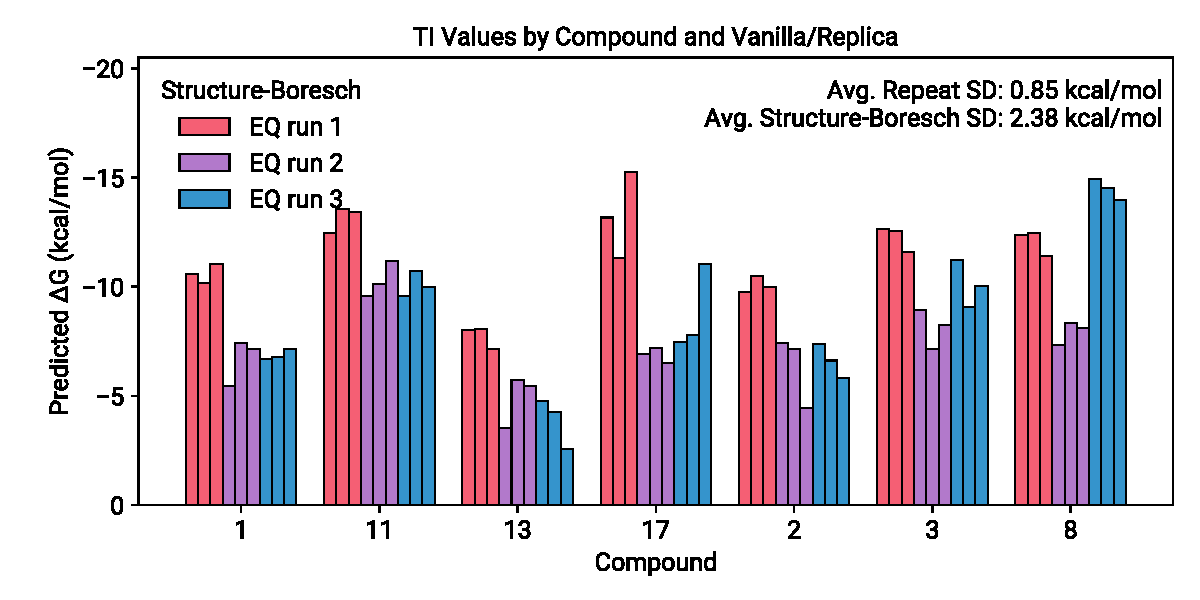
\includegraphics[width=\textwidth]{chapters/appendixA/figures/si_s2/si_figure_S2.pdf}
  \caption[Repeat-level Lenselink ABFE estimates by Boresch restraint setup.]{Predicted absolute binding free energies for the Lenselink dataset. Individual bars show repeated ABFE calculations, coloured by Boresch restraint--structure setup. Variability between different setups exceeds variability between repeats within the same setup.}
  \label{fig:si-boresch-repeats}
  \caption*{Reproduced from SI Figure S2 of Anand et al.\cite{anand2026improving} under CC BY 4.0.}
\end{figure}
\clearpage
\section{Establishing the Sampling protocol}
We first evaluated Absolute Binding Free Energy (ABFE) calculations on membrane protein systems well-characterized by relative binding free energies (RBFE). This approach minimizes errors from binding conformations and force fields, while allowing a direct comparison with RBFEs. Using a system with known RBFE performance also helps isolate ABFE-specific errors, such as assumptions about the apo-state conformation. For our initial study, we selected the Lenselink et al. (13) adenosine A2A receptor (A2A) data set, where in a recent study (19) RBFE calculations captured the maximal experimental variance (compared to 12 other GPCR systems) with an R2 of 0.84. We first assessed the performance of four different sampling strategies on this data set to establish the likely best protocol for ABFE calculations going forward.
\begin{figure}[htbp]
  \centering
  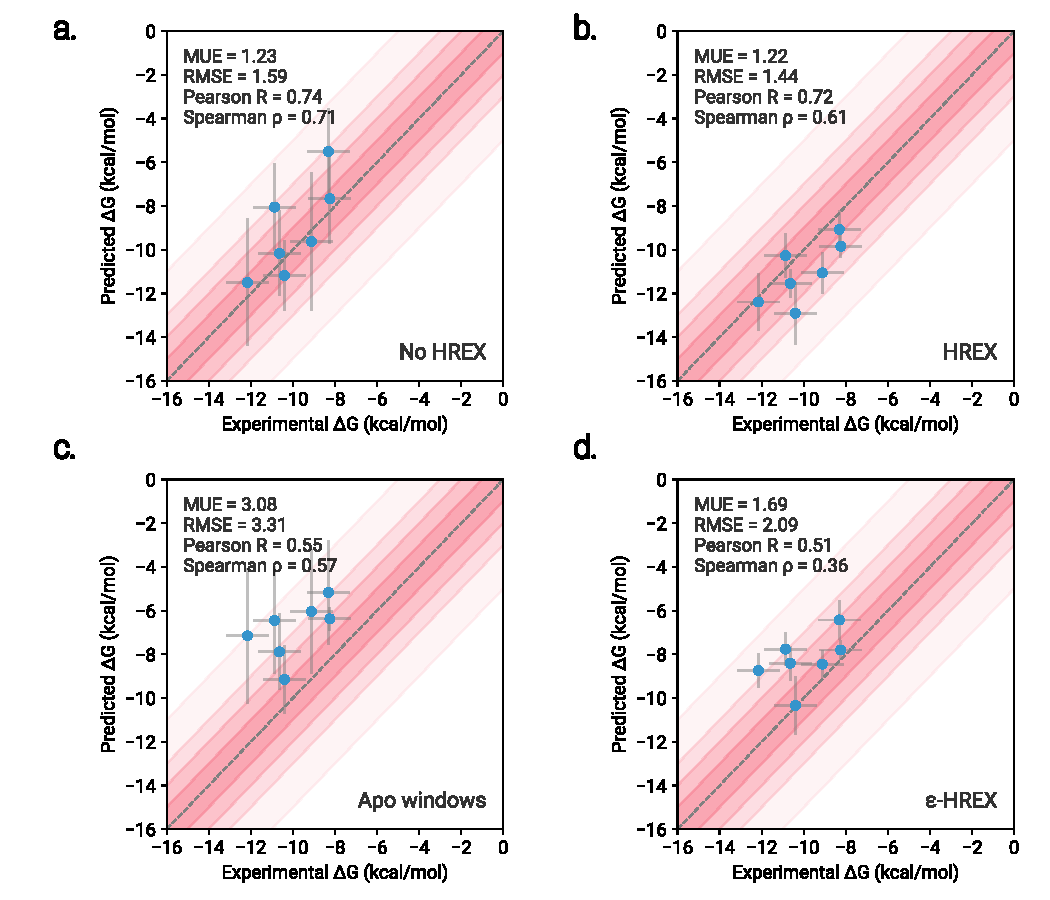
\includegraphics[width=\textwidth]{chapters/Ch3-Benchmarking-and-System-preparation/figures/combined_square_v3.pdf}
  \caption[Comparison of sampling protocols for absolute binding free-energy calculations.]{Experimental and predicted binding free energies for seven ligands using (a) no Hamiltonian replica exchange (HREX), (b) HREX, (c) apo windows, and (d) $\epsilon$-HREX. Points show mean predictions across repeats; vertical error bars show the standard deviation across repeats, and horizontal error bars indicate an assumed experimental uncertainty of $1\,\mathrm{kcal\,mol^{-1}}$. The dashed line indicates perfect agreement, and shaded bands mark deviations of $\pm 1$, $\pm 2$, $\pm 3$, and $\pm 5\,\mathrm{kcal\,mol^{-1}}$.}
  \label{fig:benchmark-sampling-comparison}
  \caption*{Reproduced from Figure 1 of Anand et al.\cite{anand2026improving} under CC BY 4.0.}
\end{figure}
For our baseline protocol, starting structures and Boresch (47) restraints were derived from three independent 100 ns equilibration runs. For each structure, three independent ABFE repeats were performed, resulting in nine ABFE estimates per compound across seven compounds. Comparison with experimental data from Lenselink et al. revealed that variability between ABFE estimates originating from the same Boresch-restrained structure was relatively small (see Figure S2). In contrast, the variability between estimates obtained from different Boresch-restrained structures was typically larger (Figure S2). This increased spread between distinct initial structures indicates that systematic differences associated with the choice of Boresch restraint and starting structure contribute more to ABFE uncertainty than repeat-to-repeat noise within a given setup. This higher error between different initial structures reinforces the existing best practice of using multiple different decorrelated initial structures (8, 48) to reduce error and improve sampling. When ABFE estimates were averaged across the three starting structures derived from independent equilibration simulations, agreement with experiment was good, yielding an RMSE of 1.59 kcal/mol, a Spearman ρ of 0.71, and a Pearson R of 0.74 (Figure 1a).


Having shown that statistical averaging reduces initial bias, we explored the influence of three techniques that should enhance sampling: HREX (Hamiltonian Replica Exchange) (Figure 1b), ABFEs with apo-state corrections (Figure 1c) (6, 22) and ε-HREX (Figure 1d), where the ligand’s LJ parameter, epsilon was scaled to enhance sampling. (10) ε-HREX was first introduced by Baumann et al. (35) to increase sampling in FEP calculations using the separated topology method. HREX performed best, with average standard deviation between interstructure ABFEs decreasing significantly (2.4 kcal mol–1 to 1 kcal mol–1) (Figure 1b), highlighting the benefit of exchanges between windows. A naïve Apo-state correction, (6) whereby the final 10 windows of the annihilation step are seeded from an apo state model, rather than the holo-state, did not improve the accuracy (Figure 1c). This underscores the need for a more nuanced treatment of the apo state (see later). Naively initializing late λ windows from apo structures, especially without replica exchange, can shift the system toward an apo-like ensemble and lead to underestimated free energies. ε-HREX (Figure 1d) generally underestimated affinities, likely due to smoother epsilon scaling exploring unfavorable conformations. A complete breakdown of all individual compounds is given in SI Table S2. Based on these results, we adopted a protocol with HREX ABFEs from three starting frames obtained from three independent 100 ns equilibration simulations and used this as the default for the remainder of the paper.




Repeat-level estimates grouped by Boresch restraint--structure setup are shown in
Figure~\ref{fig:si-boresch-repeats}.


\section{Effect of Allosteric Sodium}:

Table of how much experimental evidence for ions and how they are handles:

\begin{table}[htbp]
    \centering
    \caption{Evidence for sodium ion binding in GPCRs.}
    \label{tab:gpcr_sodium_evidence}
    \begin{tabular}{lccc}
        \hline
        \textbf{GPCR} & \textbf{Computational} & \textbf{Functional} & \textbf{Structural} \\
        \hline
        A$_{2A}$  & Yes & Yes & Yes \\
        OX$_2$R   & No  & No  & No  \\
        TAAR1     & No  & No  & No  \\
        mGlu$_5$  & No  & No  & No  \\
        DOR       & Yes & Yes & Yes \\
        D$_3$R    & Yes & Yes & No  \\
        \hline
    \end{tabular}
\end{table}



Experimental evidence and used so we look at the effect of ions:



A2A, OX2R and D3

in A2A and DOR, Resolved but in D3 and OX2R no resolved. mGlu5 is different family all togehter. 





Allosteric Sodium as a Source of Systematic Bias in A2A ABFE Calculations
Biologically abundant metal ions such as Na+, Mg2+, Ca2+ and Zn2+ have been known to modulate GPCR activity by stabilizing the receptor’s inactive state and thereby preventing receptor activation. Among these, Na+ has been extensively characterized as an endogenous negative allosteric modulator for many class A GPCRs. (50) The allosteric Na+ typically occupies a binding pocket within the transmembrane domain, located near the highly conserved Asp (2, 50) and is known to form a coordination network involving surrounding polar residues and structured water molecules. (50)

Structural studies of the A2A adenosine receptor have resolved a Na+ binding site (51) that coordinates residues such as Ser3.39 and Asp2.50. In contrast, for some receptors such as the dopamine D3 Receptor, although sodium has been shown to modulate ligand binding, there is no direct experimental resolution of the ion in available structures. For other receptors like mGlu5, the role of transmembrane ion binding in modulating receptor activity remains largely unexplored.

As a consequence of the uneven experimental characterization of ion binding sites, the treatment of ions during system preparation for free-energy perturbation (FEP) calculations often varies across studies. Some computational protocols explicitly include ions in the binding pocket (2, 13) whereas others omit them, (21) particularly when a reasonable agreement with experimental data is obtained without their inclusion. This variability is evident in the calculations performed by Guo et al. While the A2A receptor systems with ligands from Minetti, Piersanti and Deflorian explicitly included the Na+ ion, those from Lenselink et al. did not include them. Notably, despite the absence of the sodium, the Lenselink data set exhibited the highest correlation with experimental binding affinities (R (2) = 0.84) among all data sets analyzed by Guo et al. Motivated by this apparent inconsistency, we systematically evaluated the impact of the allosteric sodium ion by performing absolute binding free energy calculations both in the presence and absence of Na+ across all the A2A systems (SI Table S4).

We see that calculations with the sodium ion always give better metrics when compared to calculations without the sodium ions for all the data sets of A2A receptor.

Figure 5 illustrates the effect of including the allosteric sodium ion on ABFE predictions across three A2A receptor data sets. For the Lenselink et al. (13) data set (Figure 5 a,b, SI Table S4), inclusion of sodium resulted in a clear improvement in predictive performance, reducing the mean unsigned error (MUE) from 1.22 to 0.91 kcal mol–1 and the RMSE from 1.44 to 1.08 kcal mol–1. Improvements were also observed in correlation metrics, with the Pearson and Spearman coefficients increasing from 0.72 to 0.90 and from 0.61 to 0.82, respectively.

A similar trend was observed for the Minetti et al. (52) data set (Figure 5 c,d, SI Table S4). Inclusion of sodium substantially improved accuracy, with the MUE decreasing from 2.22 to 1.22 kcal mol–1 and the RMSE from 2.54 to 1.41 kcal mol–1. Corresponding improvements in correlation metrics were also observed, indicating better ranking of compounds.

For the Deflorian et al. (2) data set (Figure 5 e,f, SI Table S4), which spans a narrower experimental affinity range, inclusion of sodium again led to improved agreement with experiment. In this case, a pronounced reduction in the overestimation of binding affinities was observed, with the MUE decreasing from 5.48 to 2.95 kcal mol–1 and the RMSE from 5.53 to 3.05 kcal mol–1. These results suggest that explicit inclusion of sodium preferentially stabilizes the apo receptor state, thereby shifting the conformational ensemble away from an inactivated (holo-like) state toward an heterogeneous apo-like state more consistent with experimental binding measurements.

Although a reduction in correlation coefficients was observed, they remained high overall, with the Pearson correlation decreasing from 0.97 in the absence of sodium to 0.88 when sodium was included.

Allosteric Sodium as a Source of Systematic Bias in ABFE Calculations of the D3 Receptor
Like other class A GPCRs, the dopamine D3 receptor (D3R) contains a conserved allosteric Na+ binding site located beneath the orthosteric pocket. This site is centered on Asp2.50 (Asp72 in D3R numbering) and coordinates a network of water molecules via the side-chain carboxylate of Asp2.50 and the hydroxyl group of Ser3.39 (Ser114 in D3R). Although no experimental D3R structure has been resolved with a bound sodium ion, the cavity observed in the eticlopride-bound D3R crystal structure (53) closely superimposes with Na+ binding sites identified in other aminergic GPCRs, including the β1- and β2-adrenergic and A2A adenosine receptors. To validate the functional role of the cavity, Michino et al. (54) explicitly modeled Na+ into this cavity and performed long-timescale molecular dynamics simulations of the resulting D3R–ligand complexes. In these simulations, the ion remained stably coordinated with sodium binding stabilizing a specific rotameric state of Ser (3, 39) leading to a stabilized inactive-like conformation of the binding pocket. In contrast, simulations performed in the absence of Na+ exhibited increased conformational heterogeneity of side chain movement.

Experimental studies have further demonstrated that sodium ions enhance the binding affinity of D3R for several antagonists and inverse agonists, including SB-277011-A, L-741,626, GR103691, and U99194. (55, 56) In contrast, the affinities of some ligands like spiperone and (+)-butaclamol appear insensitive to sodium while the affinity of other ligands like clozapine seems to be sensitive to the overall ionic strength rather than to specific cation effects. Although these compounds are structurally distinct from the SAR series reported by Kumar et al., (56) (SI Table S5), the documented sodium dependence of several known antagonists together with the absence of a resolved Na+ ion in the structures reported by Guo et al. motivated us to examine the role of sodium binding in modulating D3R ligand affinity. Therefore, we performed absolute binding free energy (ABFE) calculations using receptor models with and without a bound Na+ ion. The Na+ -bound D3R model was generated by transferring the ion from the A2A receptor structure (PDB ID: 4EIY) (57) into our D3R model after superimposing the structures.

ABFE calculations performed with Na+ unbound (Figure 6a) and Na+ bound (Figure 6b) systems show comparable performance, with RMSE values of 2.93 and 2.94 kcal/mol, respectively. The Na+ bound system yields marginally better absolute error (MUE of 2.22 vs 2.33 kcal/mol) but slightly worse linear agreement (Pearson R of 0.34 vs 0.41), while compound ranking remains identical (Spearman ρ = 0.43 in both cases). Overall, Na+ inclusion has a small effect on D3 receptor calculations, with no observed drawback, though the small sample size limits the strength of this conclusion.

These results align with the established role of Na+ in entropically stabilizing the apo receptor, which is expected to reduce antagonist binding affinity and mitigate the observed overestimation of ABFE values. Therefore, from these results for the A2A and D3 receptors, we conclude that while including suspected bound ions is advisable, this cannot be universally generalized and should be applied with caution on a system-by-system basis (see SI Table S6).

\begin{figure}[p]
  \centering
  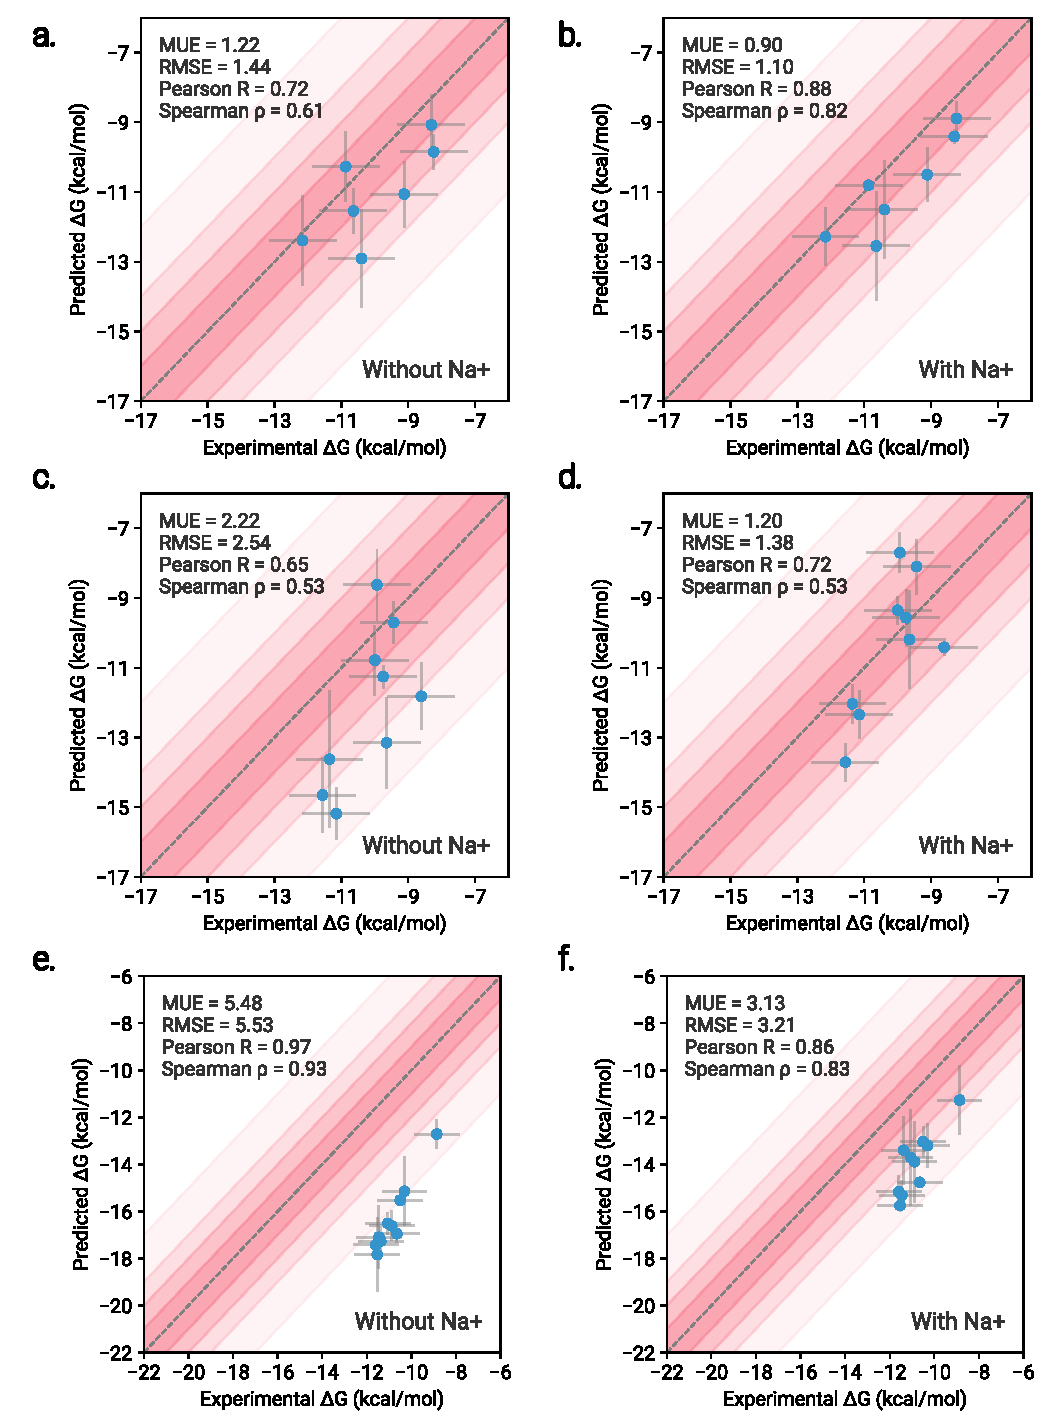
\includegraphics[width=\textwidth,height=0.72\textheight,keepaspectratio]{chapters/Ch3-Benchmarking-and-System-preparation/figures/allosteric_sodium/paper_figure_5.pdf}
  \caption[Effect of allosteric sodium on calculated binding free energies.]{Effect of allosteric sodium on calculated binding free energies for the Lenselink (a, b), Minetti (c, d), and Deflorian (e, f) A$_{2A}$ receptor datasets, without (left) and with (right) Na$^{+}$. Points show mean calculated binding free energies; vertical error bars show the standard deviation across repeats, and horizontal error bars are set to $1$~kcal~mol$^{-1}$. Dashed lines indicate agreement with experiment; shaded bands mark deviations of $1$, $2$, $3$, and $5$~kcal~mol$^{-1}$. Panels report mean unsigned error (MUE), root mean square error (RMSE), Pearson $R$, and Spearman $\rho$.}
  \label{fig:allosteric-sodium}
  \caption*{Reproduced from Figure 5 of Anand et al.\cite{anand2026improving} under CC BY 4.0.}
\end{figure}

Supplementary water-occupancy comparisons, Lenselink resolvation results, and
pooled A$_{2A}$ predictions are provided in
Figures~\ref{fig:si-all-datasets-water-occupancy}, \ref{fig:si-lenselink-gcmc},
and~\ref{fig:si-combined-a2a}, respectively.

\subsection{Deflorian OX2R}

\lipsum[1][1-3]

\subsection{Lenselink A2A}

\lipsum[1][1-3]

\subsection{Minetti A2A}

\lipsum[1][1-3]

\subsection{Piersanti A2A}

\lipsum[1][1-3]

\subsection{Deflorian A2A}

\lipsum[1][1-3]

\subsection{Kumar D3}


\begin{figure}[htbp]
  \centering
  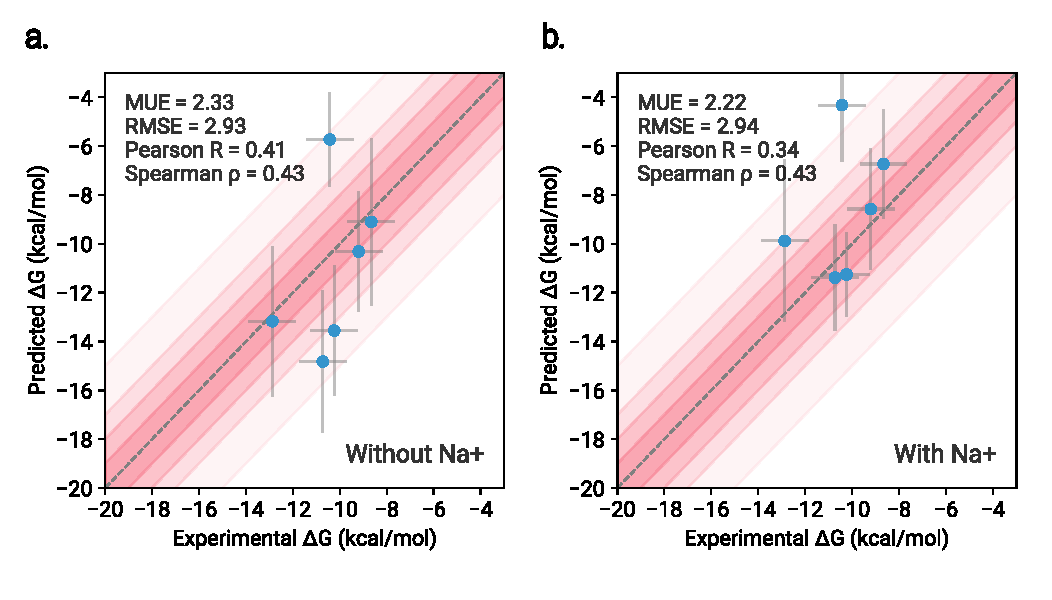
\includegraphics[width=\textwidth]{chapters/Ch3-Benchmarking-and-System-preparation/figures/figure_3_3/combined_v4_converged.pdf}
  \caption[Effect of sodium on Kumar D3 binding-affinity predictions.]{Experimental and predicted binding free energies for the Kumar D3 dataset (a) without and (b) with sodium. Points show mean predictions; vertical error bars show the standard deviation across repeats, and horizontal error bars show an assigned experimental uncertainty of $1\,\mathrm{kcal\,mol^{-1}}$. The dashed line indicates agreement with experiment; shaded bands mark deviations of $1$, $2$, $3$, and $5\,\mathrm{kcal\,mol^{-1}}$.}
  \label{fig:kumar-d3-sodium}
  \caption*{Reproduced from Figure 6 of Anand et al.\cite{anand2026improving} under CC BY 4.0.}
\end{figure}

\lipsum[1][1-3]


\section{Conclusions}
% TODO: Add content here.
\lipsum[1][1-3]
